% !TeX root = Protokoll.tex

Die Durchführung des Versuchs besteht aus der schrittweisen Erstellung des in \cref{fig:diodenlaser_aufbau_nr}
gezeigten Versuchsaufbaus, der es ermöglicht mit Hilfe des Diodenlasers das Absorptionsspektrum
von Rubidium aufzunehmen. Im Folgenden wird dieser Aufbau und die dafür verwendeten Bauteile 
mit Bezug auf die physikalischen Vorgänge im Diodenlaser im Detail erläutert.

\FloatBarrier
\begin{figure}[!h]
\centering
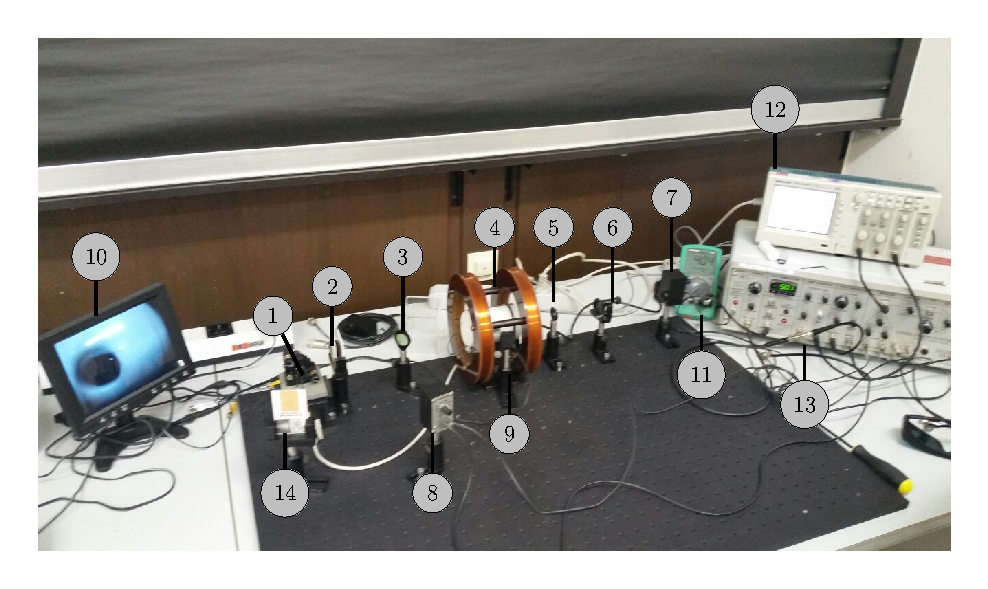
\includegraphics[scale=1]{../Grafiken/Diodenlaser_Aufbau_Nr.pdf}
\caption{Vollständiger Aufbau nach Durchführung des Versuchs, mit dem das Absorptionsspektrum von 
	Rubidium aufgenommen wurde. Die nummerierten Bauteile sind im Einzelnen:
	(1) Diodenlaser \& Gitter, (2) ND-Filter, (3) Strahlteiler 50:50, (4) Rubidiumkammer,
	(5) Blende, (6) ND-Filter, (7) Photodiode, (8) Photodiode, (9) Kamera, (10) Kamera-Monitor,
	(11) Voltmeter, (12) Digitales Oszilloskop, (13) Steuerungseinheit, (14) IR-Sichtkarte.
	\label{fig:diodenlaser_aufbau_nr}}
\end{figure}
\FloatBarrier

\subsection{Einstellung des Diodenstroms} \label{sec:einstellung_diodenstrom}
Vor Beginn der Montage der Bauteile auf dem optischen Tisch wird der Diodenlaser zum lasen gebracht.
Die dafür notwendige Besetzungsinversion wird durch den Strom erzeugt der durch die Laserdiode 
fließt. Eingestellt werden kann dieser an der Steuereinheit (13) in \cref{fig:diodenlaser_aufbau_nr} und
kann über einen Widerstand von $R_{I} = \SI{100}{\ohm}$ mit dem Voltmeter (11) nach
$I = U_{I} \cdot {R_{I}}^{-1}$ abgelesen werden. 
Der Zustand des Lasers wird mit Hilfe der IR-Sichtkarte (14) überprüft, diese wird in den Strahlengang 
gestellt und von der Rückseite mit der Kamera (9) aufgenommen und auf dem Monitor (10) beobachtet.
In \cref{fig:diodenlaser_zustand} sind zwei Aufnahmen gezeigt, die den Unterschied zwischen dem Lasen und der 
Emission von nicht kohärentem Licht verdeutlichen.

\FloatBarrier
\begin{figure}[!h]
\centering
\subfloat[Zustand in dem im Diodenlaser keine Besetzungsinversion vorliegt und das
	emittierte dem einer LED 
	gleicht. Bei einem Strom $I = \SI{30.0}{\milli\ampere}$ aufgenommen.
	\label{fig:diodenlaser_aus}]{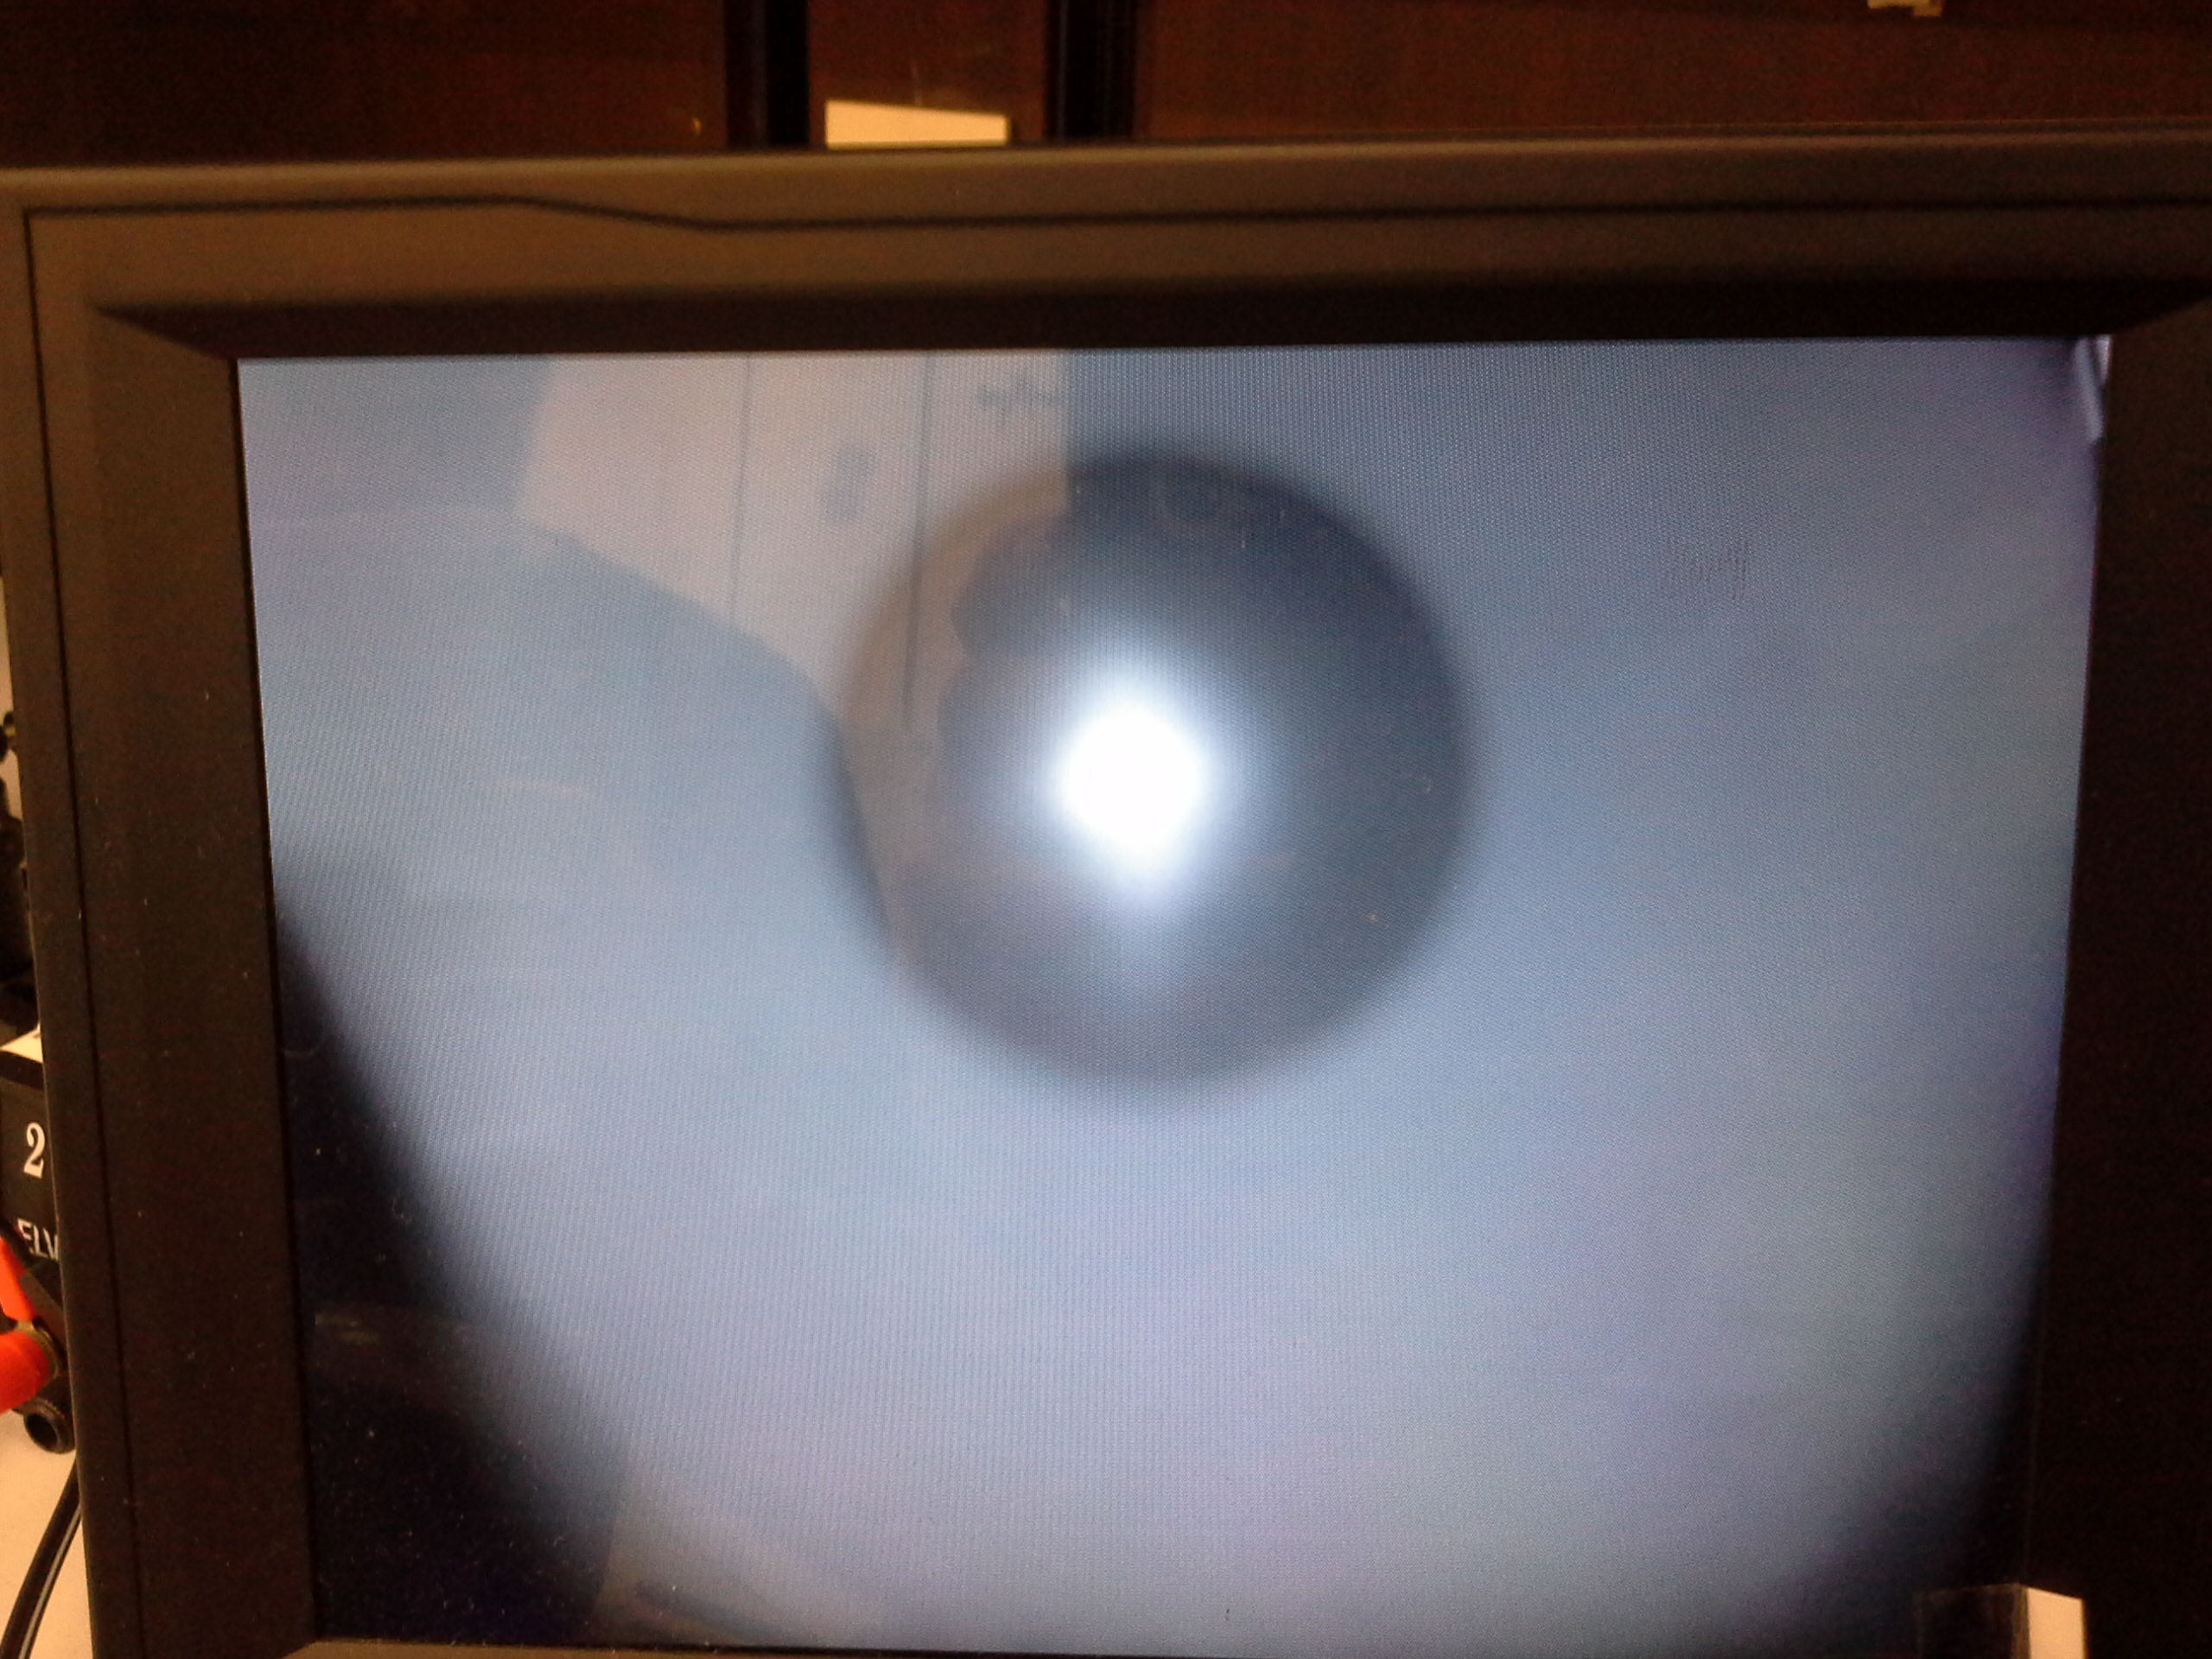
\includegraphics[scale=0.08]{../Grafiken/Diodenlaser_aus.jpg}}
\qquad
\subfloat[Zustand in dem im Diodenlaser Besetzungsinversion vorliegt und dieser zu lasen beginnt.
Das es sich bei dem hier zu beobachtenden Schein um kohärente Licht handelt ist an den einzeln
zu erkennenden Leuchtpunkten (den sogenannten speckles) am Rand des Strahles zu erkennen.
An der geringsten Strom $I = \SI{30.4}{\milli\ampere}$ aufgenommen, bei dem der Laser noch
zum lasen gebracht werden konnte.
\label{fig:diodenlaser_an}]{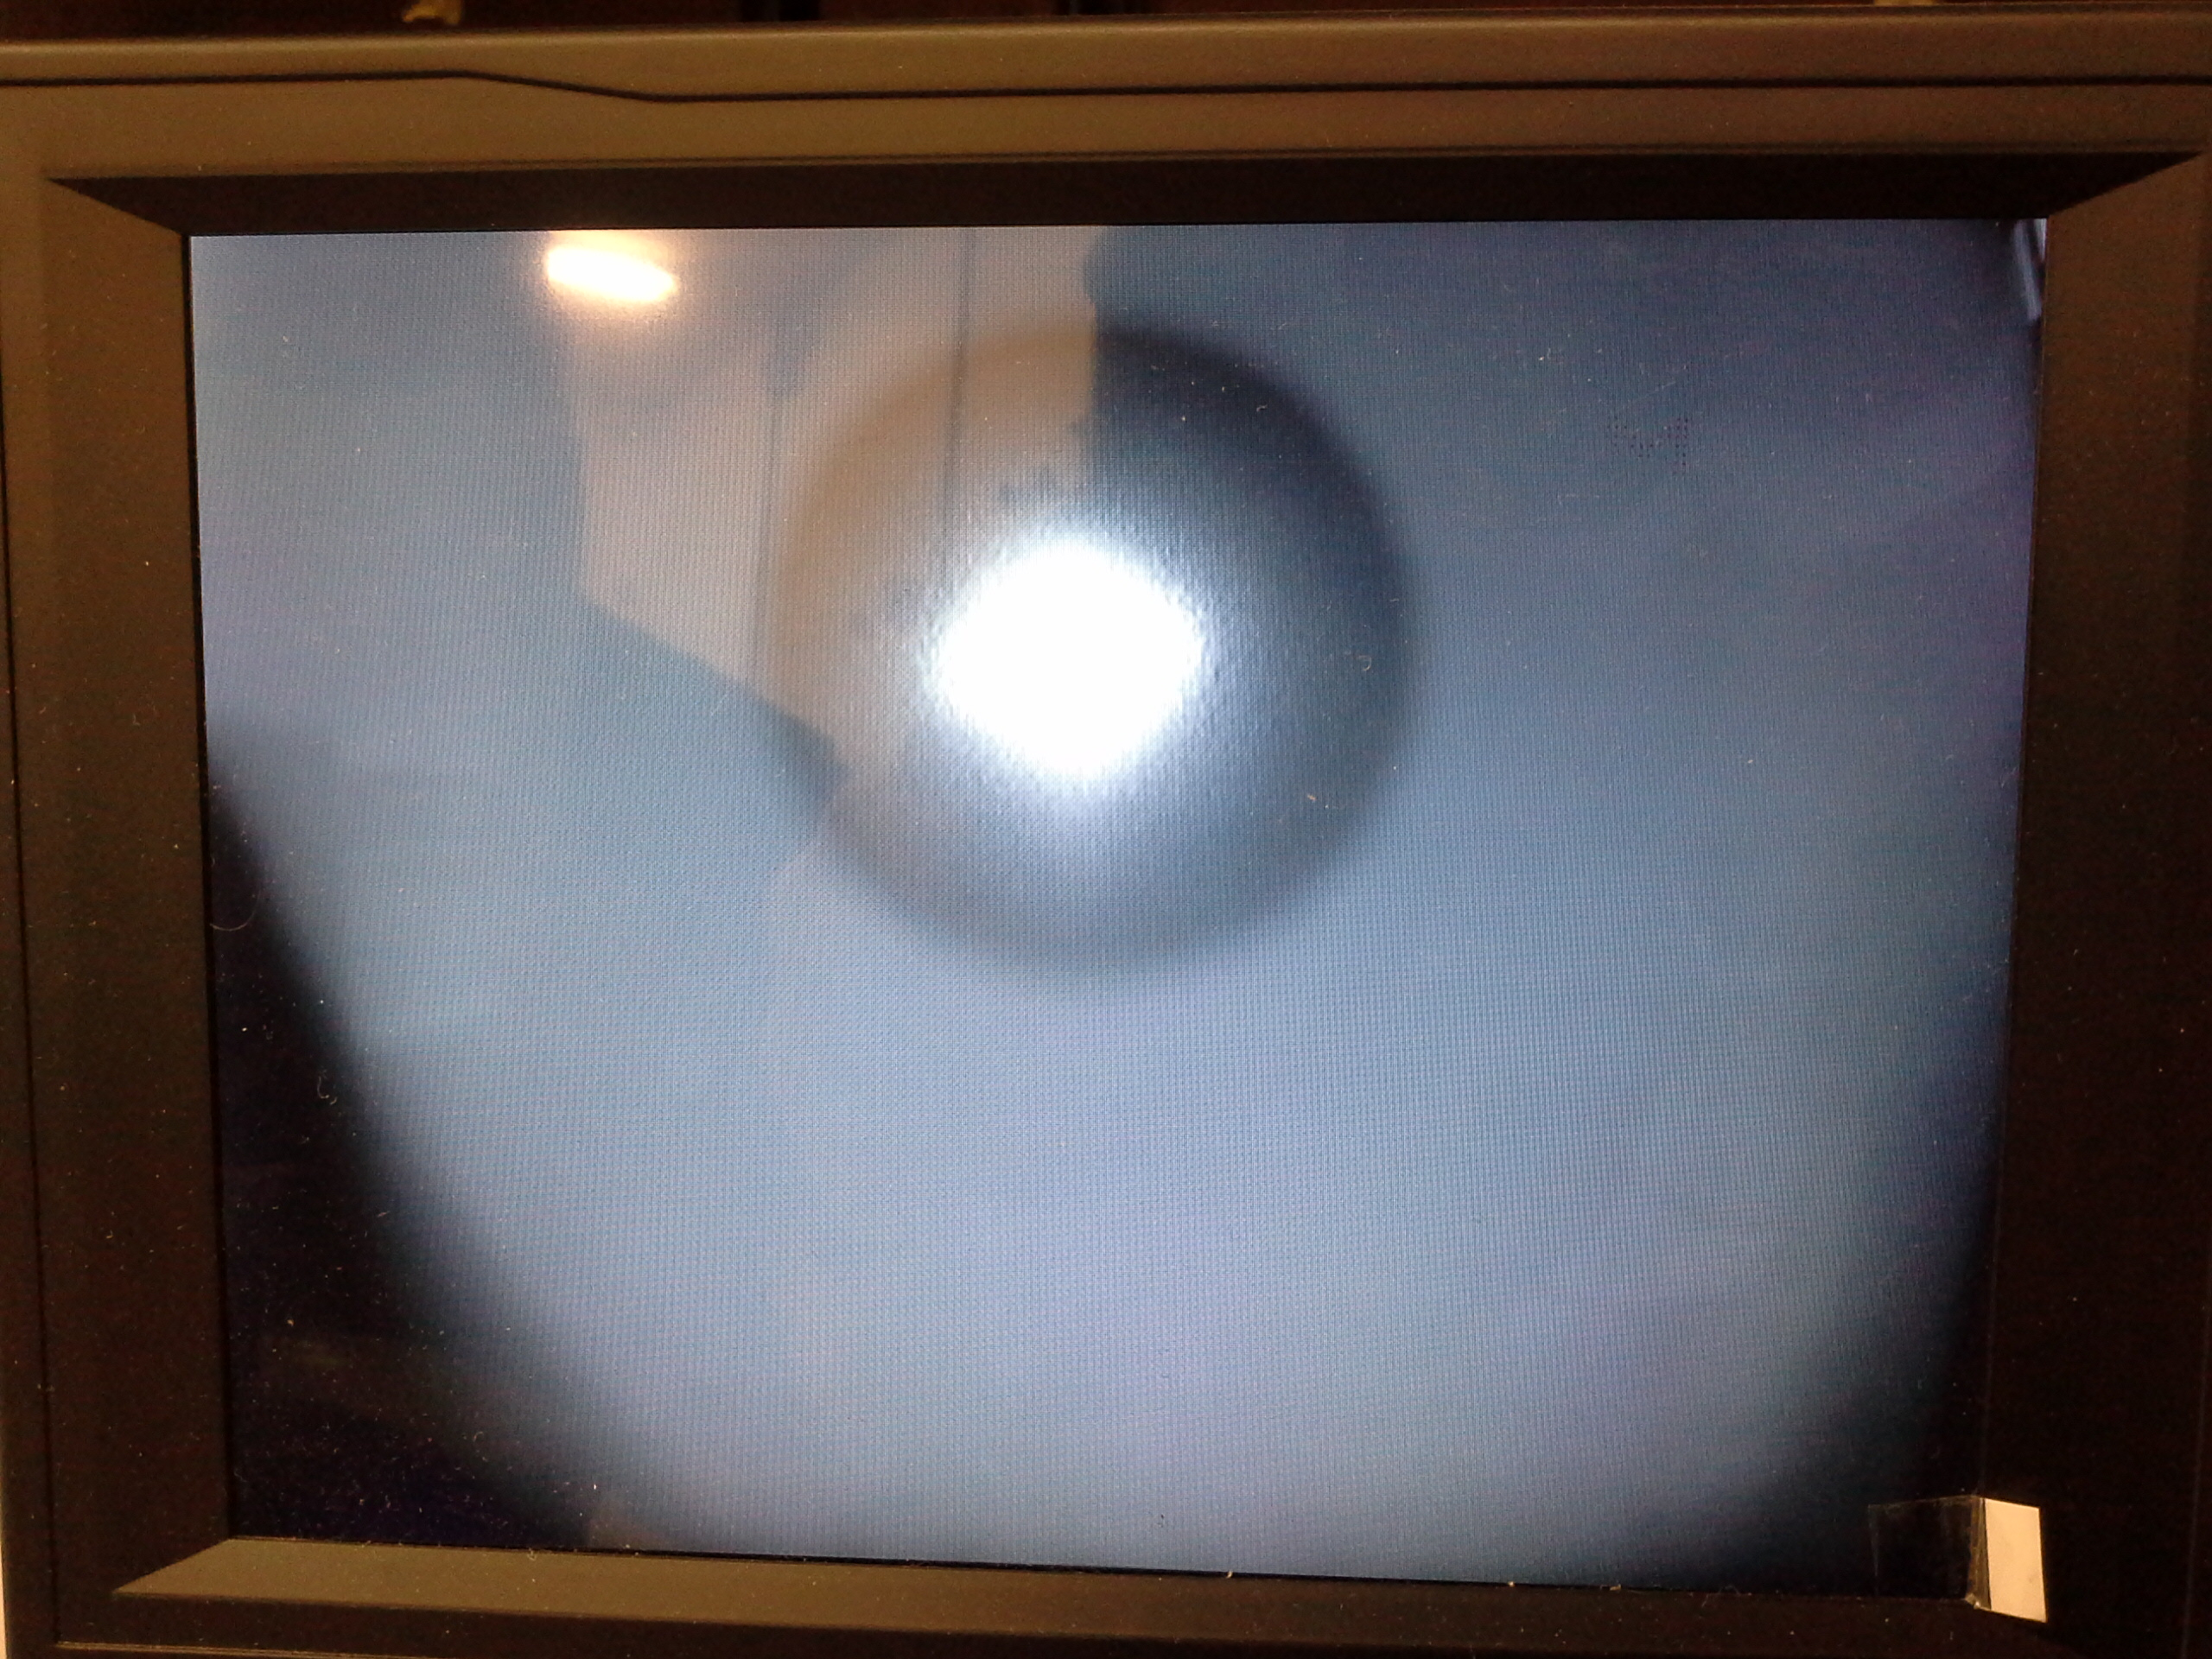
\includegraphics[scale=0.08]{../Grafiken/Diodenlaser_an.jpg}}

\caption{Bilder der beiden unterschiedlichen Emissionsarten des Diodenlasers, durch eine IR-Sichtkarte 
	sichtbar gemacht.\label{fig:diodenlaser_zustand}}
\end{figure}
\FloatBarrier

Um die interne Mode und das Maximum des Gitter-Feedbacks des Diodenlasers auf eine möglichst 
geringe Wellenlänge einzustellen ist es notwendig den Strom der durch die Diode fließt so weit 
wie möglich zu verringern.
Dies wird in mehreren Schritten erreicht nachdem der Strom so eingestellt wurde, dass 
der Diodenlaser zu lasen beginnt. In jedem Schritt wird jeweils der Strom soweit verringert,
dass der Laser gerade zu lasen aufhört. Nachfolgend wird die Güte des äußeren Resonators verbessert,
indem dieser über die Stellschrauben am Diodenlaser (1) so eingestellt wird, dass dieser erneut zu lasen beginnt. Diese Abfolge wird
so oft wiederholt wie möglich, um einen möglichst geringen Strom durch die Diode zu leiten. 

\subsection{Einstellung der Absorptionswellenlänge}
Nachfolgend wird die IR-Sichtkarte aus dem Strahlengang entfernt und Kamera wird an die 
Position auf \cref{fig:diodenlaser_aufbau_nr} gestellt, um das Innere der Rubidiumkammer (4)
zu beobachten. Durch das einfallende Laserlicht mit einer bestimmten Frequenz werden 
die Rubidiumatome angeregt und geben die dabei aufgenommene Energie über die Emission von
Photonen ab. Unter Verwendung der Kamera kann diese Fluoreszenz beobachtet werden, während
der Strom durch die Diode erhöht wird, um die entsprechende Anregungswellenlänge einzustellen.


\subsection{Einstellung des äußeren Resonators}
Um mit Hilfe des Gitters über den zu beobachtenden Wellenlängenbereich zu fahren, wird dieses
mit einem piezoelektrischen Wandler bewegt. Dieser wiederum ist an eine Dreieckspannung angeschlossen,
um eine gleichförmige periodische Bewegung in beide Richtungen (Vergrößerung und Verkleinerung des Beugungswinkels)
auszuführen. 
Die Intensität des Laserstrahls hinter der Rubidium-Zelle wird nun unter Verwendung 
einer Photodiode (7) in eine Spannung 
umgewandelt, um diese neben der Piezospannung auf dem Oszilloskop anzeigen zu lassen. 
Da die Möglichkeit der Diode, Photonen aufzunehmen, begrenzt ist ergibt sich bei Einbringen
der Photodiode in den Strahlengang eines Sättigungsspannung von \SI{-11}{\volt}.
Um die Intensität des Lasers zu verringern werden verschiedene ND-Filter (Graufilter) verwendet
(2) und (6), die den Strahl gleichmäßig abdunkeln. 
Die nach Einbau der Filter mit dem Oszilloskop aufgenommenen Spannungen sind in \cref{fig:filter_und_ndfilter}
abgebildet.

\FloatBarrier
\begin{figure}[!h]
\centering
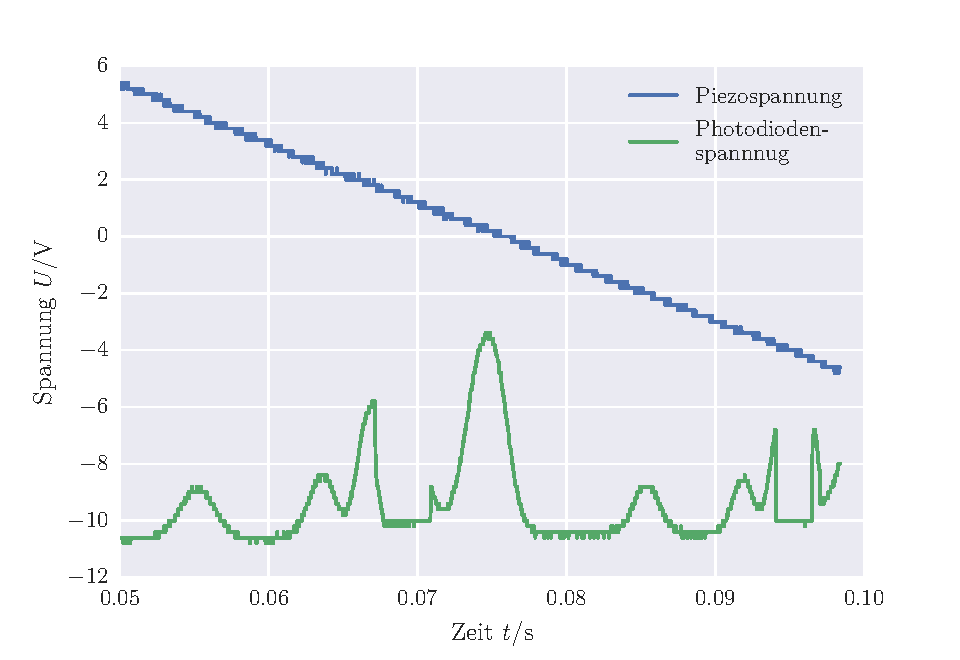
\includegraphics[scale=1]{../Grafiken/Filter_und_NDFilter.pdf}
\caption{Darstellung der vom Oszilloskop aufgenommenen Spannungen.
	 Zu sehen ist zum einen eine abfallende Flanke der an den piezoelektrischen Wandler
	 angeschlossenen Dreiecksspannung. Zum Anderen ist die Spannung der Photodiode abgebildet,
	 an der sich bereits das zu beobachtend Absorptionsspektrum erkennen lässt.
	 Neben den Absorptionsspitzen sind auch die noch vorhandenen Modensprünge deutlich zu 
	 sehen.\label{fig:filter_und_ndfilter}}
\end{figure}
\FloatBarrier 

\subsection{Einstellung des inneren Resonators} \label{sec:innerer_resonator}
Die in \cref{fig:filter_und_ndfilter} hervorgehobenen Modensprünge sind der Tatsache geschuldet,
dass bei Aufnahme der Daten nur der äußere Resonator verwendet wurde, um über den zu untersuchenden
Wellenlängenbereich zu fahren. Durch zusätzliche Modulation des Diodenstroms kann auch der innere 
Resonator zum abfahren verwendet werden. Ziel ist es dabei das Abfahren des Spektrums mit beiden 
Resonatoren möglichst synchron zu durchzuführen, um einen breiten Wellenlängenbereich ohne 
Modensprünge untersuchen zu können. Die Strommodulation wird zu diesem Zwecke mit der 
selben Dreieckspannung durchgeführt, die schon an den piezoelektrischen Wandler angeschlossen wurde.
Neben dem simultanen Abfahren des Wellenlängenbereichs führt die Diodenstrommodulation auch zu 
einer Modulation der Intensität. Diese Abhängigkeit wurde schon in \cref{sec:einstellung_diodenstrom} 
festgestellt und ist dadurch zu verstehen, dass mit zunehmendem Strom die in der Diode erzeugten 
Elektronen-Loch-Paare zunehmen und durch deren Rekombination im gleichen Maße mehr Photonen
emittiert werden. Aus abnehmendem Strom folgt analog eine Verringerung der Photonenzahl. 
%Die am Oszilloskop aufgezeichnete Spannung der Photodiode ist nun proportional zu der Anzahl der 
%detektierten Photonen.
Entsprechend dieser Intensitätsveränderung erhält man den in \cref{fig:strommodulation} dargestellten
Verlauf der Photodiodenspannung. In dieser Darstellung wurde die Photodiodenspannung invertiert,
sodass ein Abnehmen der Intensität am Abfallen der Spannung zu erkennen ist.
Neben der Intensitätsveränderung zeigt sich im Vergleich mit \cref{fig:filter_und_ndfilter},
dass die Modensprünge durch die simultane Modulation von innerem und äußerem Resonator verhindert
werden konnten.

\FloatBarrier
\begin{figure}[!h]
\centering
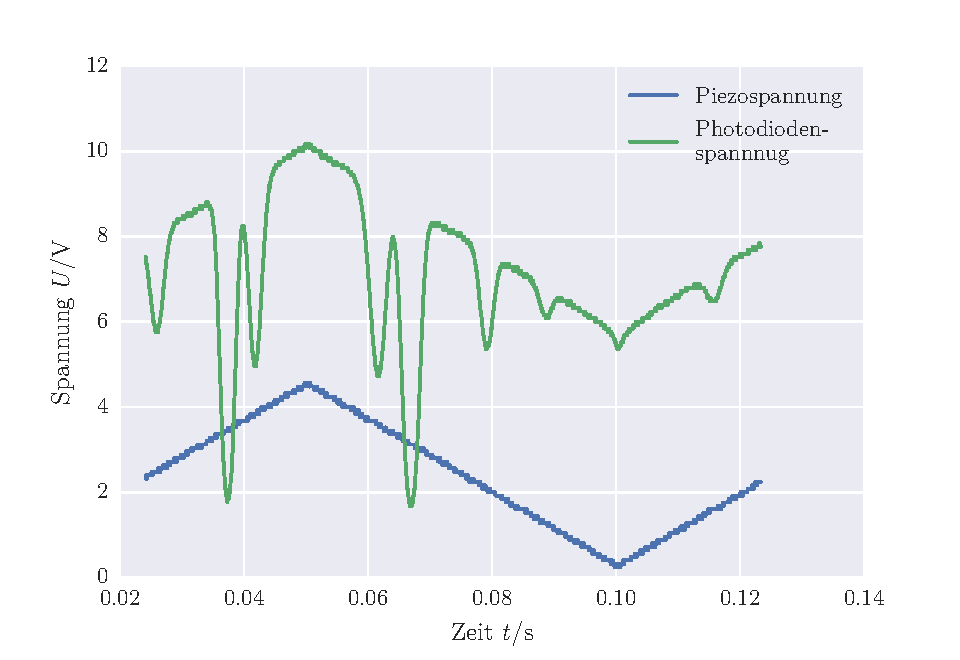
\includegraphics[scale=1]{../Grafiken/Strommodulation.pdf}
\caption{\label{fig:strommodulation}}
\end{figure}
\FloatBarrier
 

\subsection{Aufnahme des Absorptionsspektrums}

Die in \cref{sec:innerer_resonator} festgestellte Intensitätsmodulation ist für die 
Aufnahme des Absorptionsspektrums von Rubidium nicht erwünscht, da in dieser Form
beispielsweise die Tiefen der Spitzen nicht nur von der Absorption des Rubidiums,
sondern auch von der variierenden Intensität des Lasers abhängen. 
Um die Intensitätsmodulation aus dem Spektrum zu entfernen ohne dabei auf die
Strommodulation verzichten zu müssen, wird vor der Rubidiumkammer ein Strahlteiler (3) 
installiert, der \SI{50}{\percent} des Lasers durch die Kammer hindurch auf die 
bereits verwendete Photodiode fallen lässt und die übrigen \SI{50}{\percent} in
eine zweite Photodiode (8) reflektiert. Mit dieser zweiten Photodiode wird lediglich
die Intensitätsänderung durch die Strommodulation registriert, da vor dieser das 
absorbierende Rubidium fehlt. Die Spannung dieser Photodiode stellt somit eine
Nulllinie dar und kann dazu verwendet werden die Intensitätsmodulation aus dem 
Absorptionsspektrum zu entfernen. Dies geschieht durch Subtraktion der Nulllinien-Spannung
von der Spannung der erste Photodiode. Das Ergebnis dieser Subtraktion, bei der 
die Gewichte der beiden Spannungen angepasst wurden, um eventuelle Ungleichheiten in den 
Strahlintensitäten auszugleichen, ist in \cref{fig:absorptionsspektrum} in Form des Absorptionsspektrums von 
Rubidium zu sehen.
  
\FloatBarrier
\begin{figure}[!h]
\centering
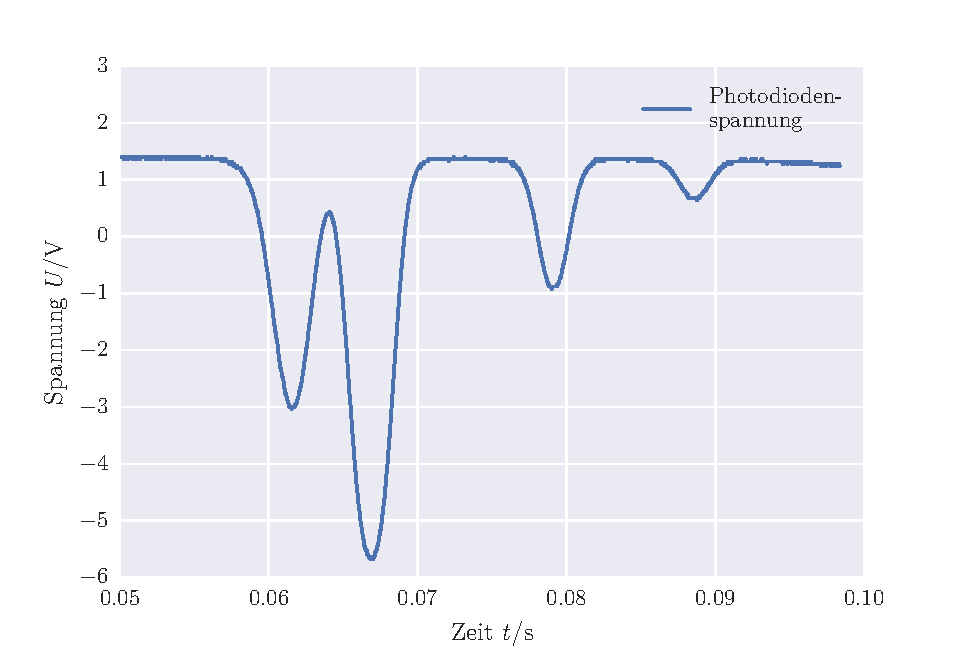
\includegraphics[scale=1]{../Grafiken/Absorptionsspektrum.pdf}
\caption{Verlauf der Differenzspannung der beiden Photodioden (vor und hinter der Rubdiumkammer).
	 Es zeigt sich das Absorptionsspektrum von Rubidium, welches detailliert genug ist, um 
	  vier unterschiedliche Isotope erkennen zu können. \label{fig:absorptionsspektrum}}
\end{figure}
\FloatBarrier  
  
\FloatBarrier
\begin{figure}[!h]
\centering
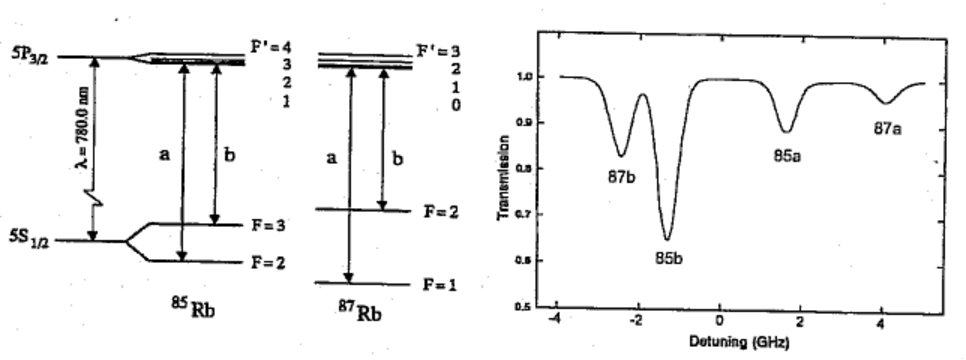
\includegraphics[scale=1]{../Grafiken/Absorptionsspektrum_Termschema.pdf}
\caption{Darstellungen der in diesem Versuch zu 
	beobachtenden Übergänge beider Rubidiumisotope 
	${}^{85}$Rb und ${}^{87}$Rb in dem jeweiligen 
	Termschema und dem entsprechenden 
	Absorptionsspektrum, welches in diesem Versuch aufgenommen wird.
	\label{fig:absorptionsspektrum_termschema}}
\end{figure}
\FloatBarrier

Das aufgenommene Absorptionsspektrum zeigt eine sehr gute Übereinstimmung mit dem theoretisch 
zu erwartenden Verlauf in \cref{fig:absorptionsspektrum_termschema}.
Sowohl in diesem als auch in dem aufgenommenen 
Spektrum sind je zwei Übergänge für die beiden 
Rubidiumisotope ${}^{85}$Rb und ${}^{87}$Rb deutlich 
zu erkennen. Aus dieser Übereinstimmung
ist zu schließen, dass sich der verwendete Diodenlaser
sehr gut für Spektroskopie von Atomübergängen, im 
entsprechenden Wellenlängenbereich, eignet.




 


